\documentclass[a4paper,11pt]{article}
%\usepackage[T1]{fontenc}

%\setlength{\textwidth}{20cm}
%\setlength{\marginparwidth}{0cm}
%\setlength{\voffset}{0cm}
\usepackage[utf8]{inputenc}
\usepackage[francais]{babel}
\usepackage{amsmath}
\usepackage{graphicx}
\usepackage{subfig}
\usepackage{hyperref}
%\special{papersize=210mm,297mm}

\newcommand{\op}{
  \mathop{
    \vphantom{\bigoplus}
    \mathchoice
      {\vcenter{\hbox{\resizebox{\widthof{$\displaystyle\bigoplus$}}{!}{$\boxplus$}}}}
      {\vcenter{\hbox{\resizebox{\widthof{$\bigoplus$}}{!}{$\boxplus$}}}}
      {\vcenter{\hbox{\resizebox{\widthof{$\scriptstyle\oplus$}}{!}{$\boxplus$}}}}
      {\vcenter{\hbox{\resizebox{\widthof{$\scriptscriptstyle\oplus$}}{!}{$\boxplus$}}}}
  }\displaylimits
}

\title{{\Huge Electronique numérique}\\Automates (1)}
\date{}

\begin{document}
\maketitle
{\it Tous les exercices ne seront pas forcément résolus en TE.}\\

Ce TD aborde plusieurs points relatifs aux {\it automates}, aussi appelés {\it machines d'états finis}
\footnote{Ce nom quelque peu étrange signifie que le {\it nombre} d'états est {\it fini}. Il existe également
des automates dont le nombre d'états est infini...}{\it finite state machines} (FSM).
\begin{itemize}
  \item Diagrammes états transitions : machines de Mealy et de Moore.
  \item Causalité des machines d'états finis.
  \item Conception d'un automate matériel à partir d'un diagramme  états-transitions.
\end{itemize}


\section{Diagramme états-transitions. Moore et Mealy}
On rappelle que le diagramme à bulle (ou ``state transition diagram'' ou diagramme ``états-transistions'') est une représentation graphique pratique des automates.
Elle consiste à décrire l'enchaînement des transitions d'un état à l'autre par une flèche,
les états étant représentés par des cercles ou ``bulles''.

On distingue deux grands types de FSM (voir figure \ref{fig:example}) \footnote{Attention !
Les deux automates représentés l'un à côté de l'autre ne sont pas équivalents en terme de fonctionnement.
Il existe des algorithmes pour transformer Mealy en Moore (et réciproquement), de manière à obtenir des
comportements identiques.... Voir par exemple \url{https://fr.wikipedia.org/wiki/Machine_de_Mealy})}. Dans le cas des automates de Moore, les sorties ne dépendent que des états, alors que dans le cas des automates de Mealy,
les sorties dépendent à la fois des états et des entrées. Sur les transitions, on ajoute les {\it conditions} booléennes $c_i(s)$ qui autorisent à passer d'un état à un autre, ainsi
que d'éventuelles sorties (généralement après une ou deux barres verticales) dans le cas des automates de Mealy. Lorsqu'on a affaire à un automate de Moore, les sorties sont annotées en
conséquence dans les bulles (ou juste à côté !).\\

\begin{figure}[!h]
    \centering
    \subfloat[label 1]{{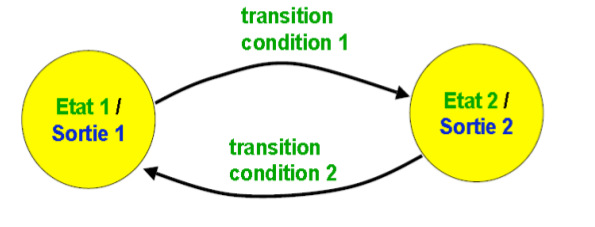
\includegraphics[width=5cm]{./figures/moore.png} }}%
    \qquad
    \subfloat[label 2]{{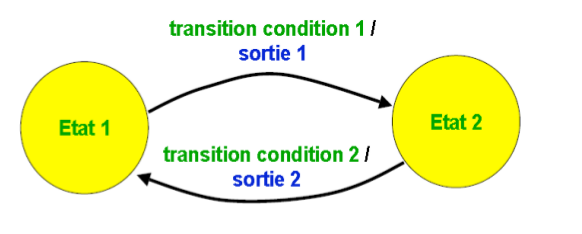
\includegraphics[width=5cm]{./figures/mealy.png} }}%
    \caption{FSM de Moore et Mealy}%
    \label{fig:example}%
\end{figure}


\section{Causalité d'une FSM}
Pour que qu'une FSM  soit considérée comme {\it causale}, correcte ou {\it consistante}, elle doit vérifier les deux propriétés suivantes :
\begin{itemize}
\item \textbf{Réactivité} (Exhaustivité des conditions): il doit exister une condition vraie sur au moins une des transitions sortant d'un état. .
$$\forall s \in S : \sum_i c_i(s)=1$$
\item \textbf{Déterminisme} (Exclusivité): deux conditions sur les transitions sortant d'un état ne peuvent être vraies en même temps.
$$\forall s \in S, \forall (i,j) \text{ avec } i \neq j, c_i(s).c_j(s)=0$$
\end{itemize}

Une autre manière de résumer ces deux propriété est qu'il existe -- à tout instant discret -- {\it un, et un seul, état suivant}.

Notons qu'un état peut avoir comme état suivant lui-même : dans ce cas, le système décrit ne change pas d'état.\\

%%$$\forall s \in S : \sum_i c_i(s)=1$$
%%$$\forall s \in S , c_1(s) \oplus c_2(s) ... \oplus c_n(S) = 1$$

%% \begin{figure}[!h]
%% \begin{center}
%% \includegraphics[scale=0.2]{./d-ff-infos.jpg}
%% \end{center}
%% \end{figure}
Observez la figure \ref{fig2}.
\begin{itemize}
\item Vérifier la consistance de la machine d'état suivante.
\item Est-ce un automate de Moore ou de Mealy ?
\end{itemize}

\begin{figure}[!h]
\begin{center}
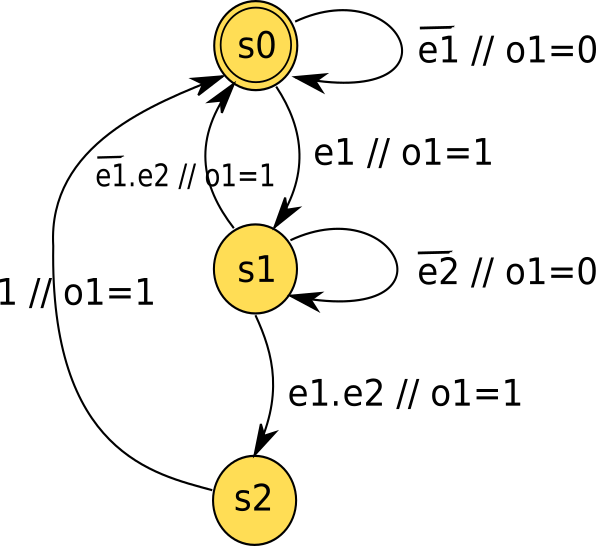
\includegraphics[scale=0.3]{./figures/ex-fsm-1.png}
\end{center}
\caption{FSM de l'exercice 1 et 2}
\label{fig2}
\end{figure}

\subsection{Equations logiques de l'automate}
On cherche les équations logiques de la fonction "état suivant", ainsi que de la fonction de sortie de l'automate précédent. Ces deux ensembles
nous permettrons de réaliser concrètement le circuit. On suggère ici de procéder en 2 étapes.
La première consiste à conserver le nom {\it symbolique} des états tandis que la seconde fait apparaître l'{\it encodage} de ces états.
Dans la FSM à réaliser, en choisissant un encodage {\it one-hot}, trois bits seraient nécessaires pour encoder les états.
On va se limiter toutefois ici à un encodage {\it dense} où 2 bits seuls sont nécessaires. On s'appuie sur les tableaux génériques suivant \ref{tab1} et \ref{tab2},
qui permettent de procéder de manière systématique.
\begin{table}[htp]

  \centering
  \caption{Encodage symbolique (nom des états préservés)}\label{tab1}

  \begin{tabular}{|l|l|l|l||l|l|l|l|}
      \hline
      état courant & entrée 1 & ... & entrée n &  état suivant & sortie 1 & ... & sortie n \\ \hline
      ~        & ~    & ~         & ~            & ~            & ~        & ~   & ~        \\
      ~        & ~   & ~     & ~            & ~            & ~        & ~   & ~        \\
      \hline
  \end{tabular}

  \bigskip

  \caption{Encodage binaire (états encodés)}\label{tab2}

  \begin{tabular}{|l|l|l|l||l|l|l|l|l|l|}
    \hline
    Q1 & Q0 &  entrée 1 & ... & entrée n & D1 & D0 & sortie 1 & ... & sortie n \\ \hline
    ~        & ~  & ~  & ~  & ~  & ~  & ~  & ~        & ~   & ~        \\
    ~        & ~  & ~  & ~  & ~  & ~  & ~  & ~        & ~   & ~        \\
    \hline
  \end{tabular}

\end{table}



\section{Application}
Soit le diagramme états-transitions de la figure \ref{exo1}. On suppose que les entrées A et B proviennent de deux capteurs.
Les sorties sont S1,S2 et S3.

\begin{figure}[!h]
  \begin{center}
    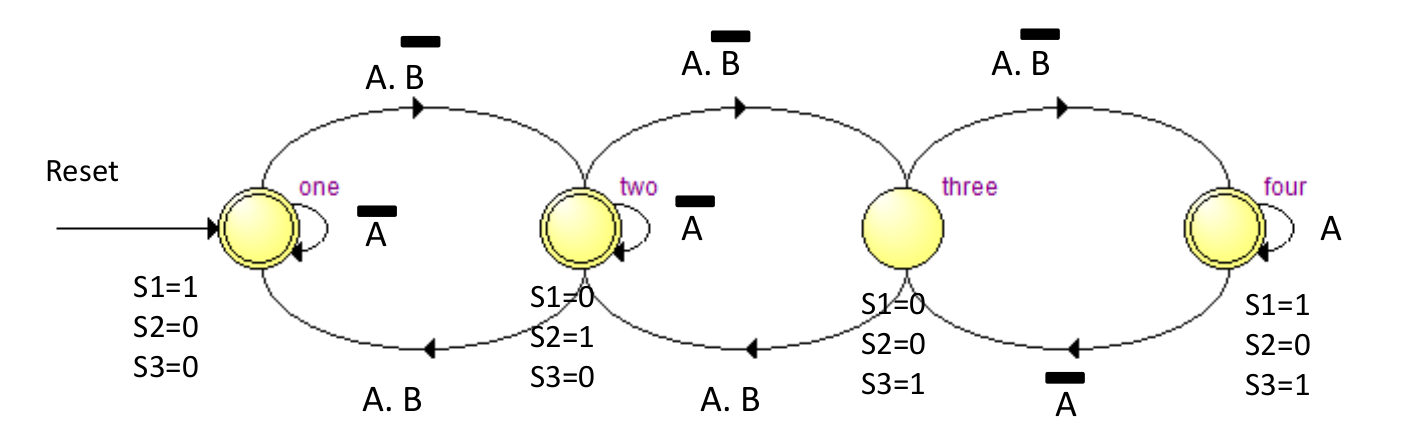
\includegraphics[scale=0.25]{./figures/exo1}
  \end{center}
  \caption{Diagramme états-transitions (à modifier).}
  \label{exo1}
\end{figure}

\begin{enumerate}
  \item Cette machine est-elle causale ? Si non, proposer une modification afin de la rendre causale.
  \item Proposer un encodage "one-hot" pour cette FSM.
  \item Etablir les équations de la fonction de transition. On rappelle que ces équations déterminent les entrées D des bascules d'état de l'automate.
  \item Etablir les équations de sortie.
  \item Dessiner la structure globale du circuit, en faisant apparaître, sous forme de nuage logique, les fonctions précédentes.
  \item Tenter de dessiner le circuit complet.
\end{enumerate}

%=================================================================================================================================
\section{Automate "détecteur de séquence"}

Il est fréquent de devoir détecter une séquence particulière dans un flux de données.
Les automates se prêtent très bien à ce genre de détection. On peut citer :
\begin{itemize}
  \item L'analyse de paquets réseaux, détection de paquets interdits (entrants ou sortants) dont on connait une certaine signature numérique. C'est le travail de filtrage d'un "proxy", etc
  \item L'analyse de flux multimedia : par exemple "start codes" de séquences, dans un film (stocké en numérique, dans un format de compression).
  \item L'analyse génomique : il existe des accélérateurs FPGA dédiés à la reconnaisance de séquence du génôme, etc.
  \item etc.
\end{itemize}

\begin{figure}[!h]
  \begin{center}
    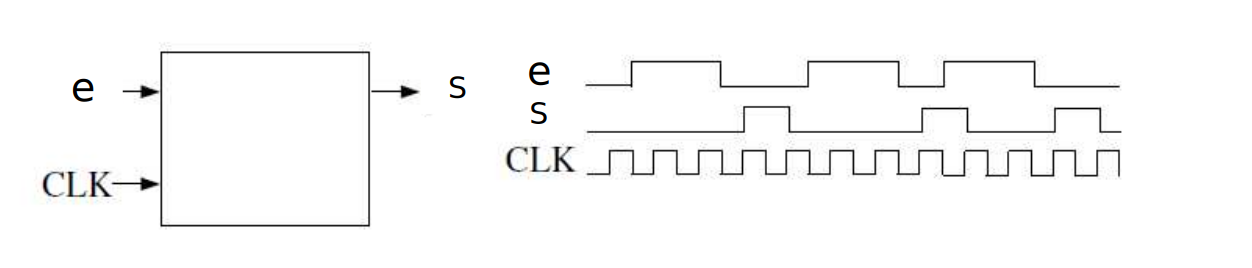
\includegraphics[scale=0.3]{./figures/exo2}
  \end{center}
  \caption{Schéma de principe du détecteur de séquence. Chronogramme associé.}
  \label{exo2}
\end{figure}

On considère le détecteur de séquence de la figure \ref{exo2}. Son rôle est de détecter les séquences "0-1-1-0" sur son unique entrée $x$.
Lorsque cette séquence est détectée, il émet un '1' sur sa sortie $y$. Un chronogramme est fourni à titre d'exemple. Notez que dans le flux
"0-1-1-0-1-1-0", la séquence apparaît deux fois !
\begin{enumerate}
  \item Proposer un diagramme états-transitions pour ce détecteur. On choisira une machine de Moore.
  \item Proposer un encodage dense des états.
  \item Réaliser le circuit.
\end{enumerate}

%=================================================================================================================================
\section{Automate "serrure numérique"}
L’accès à un local est protégé par une serrure codée associée à un
automatisme commandant la gâche électrique de la porte. La combinaison secrète est : A,D,C.

\begin{figure}[!h]
  \begin{center}
    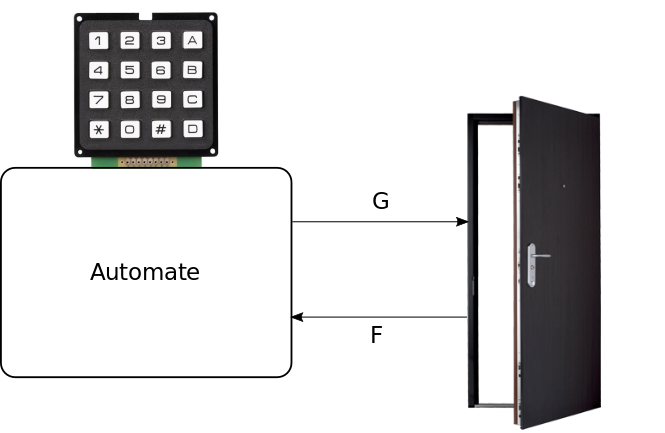
\includegraphics[scale=0.3]{./figures/porte.png}
  \end{center}
  \caption{Schéma de principe de la serrure numérique.}
  \label{exo2}
\end{figure}

Un capteur permet de connaître l'état de la porte : F indique son état. F vaut à 1 si la porte est fermée à 0 si elle est ouverte.
G commande l’ouverture de la porte : si G=1 la porte peut être ouverte. Lorsque la porte se referme, on a G=0.
A l’ initialisation la porte est fermée, le contact de porte F=1.
On précise qu'on ne peut appuyer que sur un seul bouton à la fois.

\begin{enumerate}
  \item Proposer un automate de contrôle du dispostif.
  \item Discuter de la robustesse de la solution, et de son réalisme. Proposer des alternatives.
  \item Optionel : construire le circuit complet.
\end{enumerate}

\end{document}
